% !TEX root = ../notes.tex

% ================ Data Variety ==============
\section{Data Variety}

The ``3 Vs'' of Big Data: {\it Volume}, {\it Velocity} and {\it Variety}. In this course, we don't address the {\it Volume} and {\it Velocity} parts (A course on Database does). Since there is a lot of variety in the data, we need to prepare the data. This flow is called {\bf ETL}:
\begin{itemize}
 \item {\bf Extract} from the {\it source(s)}.
 \item {\bf Transform} data at the source, sink, or in a {\it staging area}.
 \item {\bf Load} data into the {\it sink}.  
\end{itemize}
This variety of the data comes, in a first place, from the many different sources from which we extract them: {\it files, databases, logs, ... } Each of these sources uses (or not!) its proper convention and can contain structured (DB), semi-structured (logs) or unstructured (web page) data. 

\subsection{Role of Schema}
The {\bf Schema}, which specifies the {\it structure} and {\it types} of data repository, is changing. Traditional databases are {\bf schema-on-write}, {\it i.e.} you cannot load data into a table without a schema. But new data stores (NoSQL for example) are {\bf schema-on-read} or {\bf schemaless}. 

\begin{itemize}
	\item {\bf Schema-on-write} is typically SQL, where we must create a table before inserting data in our system. Data must scale the defined schema and this is both the strength and weakness of the system. Strength because the data is perfectly oriented and respect the constraints we establish. Weakness because schemas are always subjective in some ways and data (which are perfectly correct) may not fit with it. 
	\item {\bf Schema-on-read} is for instance XML, where you create the schema according to the data you read.
	\item Youtube and Google Cache where the first {\bf schemaless} data system. Without schema, everything is simply stored as a string and we need a parser to return a typed data.
\end{itemize}

\subsection{Examples of data}

\subsubsection{XML and DOM}

The XML data are used mostly with HTML and specifies the data structure. An XML schema can be applied to interpret the XML data and specifies the {\bf data types}. Figure \ref{pic:xml} shows the XML data \ref{pic:xml_data} and the schema \ref{pic:xml_schema} used to parse and type the data.

\begin{figure} [h] %----------- SubGraph ---------------------
\centerline{
\subfigure[XML data \label{pic:xml_data}] {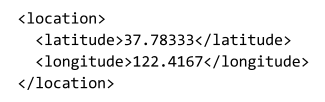
\includegraphics[width=5cm]{img/04/xml_data} }
\subfigure[XML schema\label{pic:xml_schema}] {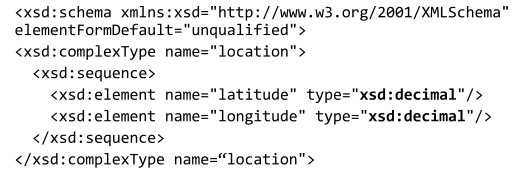
\includegraphics[width=7cm]{img/04/xml_schema} } 
}
\caption{\label{pic:xml} Example of XML.} 
\end{figure}

The XML is a text format that encodes {\bf DOM} (Document-Object Models). It's a data structure often used by Web pages. The DOM is tree-structured. An example of a DOM is given in Figure \ref{pic:dom}.

\begin{figure}[H]%---------------FIG--------------
 \centering
 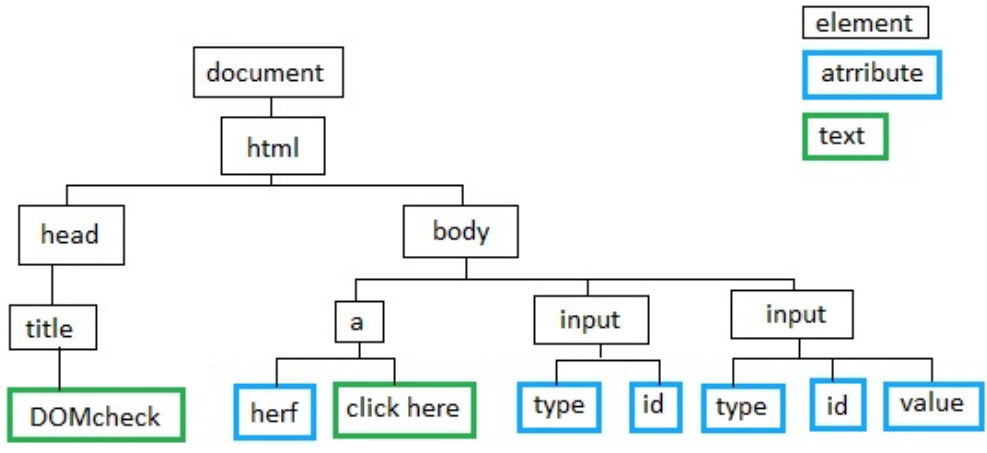
\includegraphics[width=10cm]{./img/04/dom}
 \caption{\label{pic:dom} Example of a DOM tree for an HTML Web page.}
\end{figure}

THe XML schema allows a database to interpret the data when running queries. It can do arithmetic or range queries on numerical values, for example.

\subsubsection{JSON}

{\bf JSON} stands for Javascript Object Notation. It's a schemaless data (schema support was added later). An example of JSON data is shown in Figure \ref{pic:json}

\begin{figure}[H]%---------------FIG--------------
 \centering
 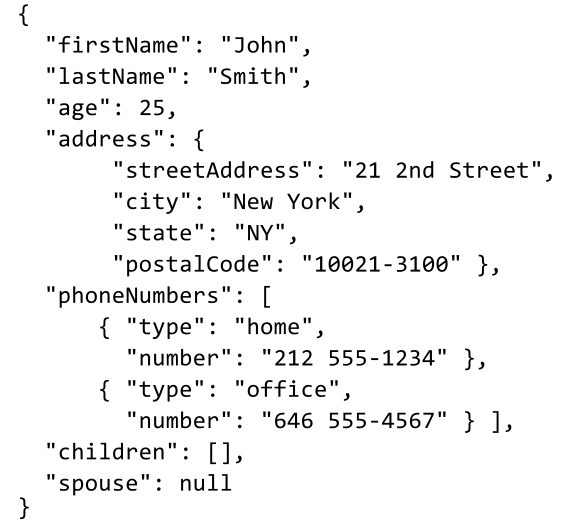
\includegraphics[width=8cm]{./img/04/json}
 \caption{\label{pic:json} Example of a JSON data.}
\end{figure}

JSON is typically used to represent {\bf hierarchical data structures} directly in the target language (Javascript or Java at the beginning). The transformation on the data is procedural in the target languages. It is often easier for some tasks, but it can be painful for some of them: for example schema changes.

\subsubsection{Tabular data}

A Tabular Data is simply data put into a table such as CSV or TSV. Definition of a table:
\begin{itemize}
 \item A {\bf table} is a collection of {\bf rows} and {\bf columns}.
 \item Each row has an {\bf index}.
 \item Each column has a {\bf name}.
 \item A {\bf cell} is specified by an (index, name) pair.
 \item A cell may or may not have a {\bf value}.
\end{itemize}

It's a very simple yet powerful data type. For example, the sensors usually output data in the form of time series, transformed into a tabular format. However, a system dealing with sensor data should:
\begin{itemize}
 \item support both long-term ({\bf trend}) and short-term ({\bf real-time}) queries
 \item have {\bf low latency} but also efficient. It should use {\bf real-time indexing} for longer-term queries.
 \item support triggers ({\bf alerts}) for a variety of conditions.
\end{itemize}
Therefore, the {\bf complexity of a data format} does not determine the {\bf complexity of the system required to properly handle it}.

\subsubsection{Log files}

The log files are simple text files giving information about the process. The daemons, such as \verb+httpd+, \verb+mysqld+ or \verb+syslogd+, usually create logs. {\bf \verb+syslog+} was developed by Eric Allman. It's a way for devices to send event messages to a server that will log all the events. Splunk is a company that built a successful business model around the syslog events.

\subsubsection{Binary formats}

They are often the key to performance because we {\bf avoid expensive parsing}. The modern formats even support nested structures, various levels of schema enforcement, {\bf compression}, etc. Some examples: Protocol Buffers (Google), Avro, Parquet, etc.

\subsection{Processing the data (JSON and XML)}

In order to process XML, we can use the DOM. It can also be used to process JSON data. The DOM is very easy to work with: all the data are directly accessible by links. The problem is that we {\bf might not care about most of the data} and if the data are big, they {\bf might not fit into the RAM}. In order to deal with these two problems, we can use a {\bf SAX} parser which is an event-driven parser. It will find all the {\bf open-close-tag events} in an XML document and will {bf do callbacks to user code}.

\begin{itemize}
\renewcommand{\labelitemi}{{\bf +}}
 \item User code can respond to only a subset of events corresponding to the tag it is interested in.
 \item User code can correctly compute aggregates from the data rather than create a record for each tag.
 \item User code can implement flexible error recovery strategies for ill-formed XML.
\renewcommand{\labelitemi}{{\bf --}}
 \item User code must implement a state machine to keep track of ``where it is'' in the DOM tree.
\end{itemize}

For JSON, most parsers construct the ``DOM'' directly. But there are a few SAX-style parsers: Jackson, JSON-simple, etc. Sometimes {\bf SAX-style is the way to handle ill-formed datasets}, an endless array of objects, for example.

\subsection{HTML and Web Services}

\subsubsection{HTML}

Internet contains an ``enormous'' amount of data. Some crawlers such as Common Crawl datasets contains about 1.82 billion web pages (for 145 TB). We can use different tools to crawl data from the web. Examples for Python: Beautiful Soup, Requests, Scrapy, etc. 
\\\\
Most of the time, the Web pages are considered as unstructured data. But you can find some semi-structured data, {\it e.g.} Google WebTables. Some big ``internet'' companies (Google, Yahoo, Yandex and Microsoft) are sponsoring a project called {\bf schema.org} to create structured or semi-structured Web pages. A core vocabulary for the type of fields is given. schema.org is more and more used. It's also used by knowledge bases such as Google Knowledge Graph. {\bf WikiData} is a community project to create an open database of structured data taken from Wikipedia.

\subsubsection{Web Services}

Screen-scraping the content of a large website was possible before, but become more and more difficult nowadays. This is mainly due to the content "hidden" behind a form or an authentification. Take for example facebook without account, or the IS-academia course page if you do not select a semester. Therefore big companies are providing Web Service APIs\footnote{Application Program Interface: Set of subroutine definitions, protocols, and tools for building software and applications. In this particular case, the APIs are used to retrieve the data from the Web page, {\it e.g.} Facebook API to retrieve the contacts.} to retrieve data from their website. There are two kinds of Web Services:
\begin{itemize}
 \item The old way: XML-based RPC-style messages: SOAP
 \item The new way: REST-style stateless interactions, URLs encode state
\end{itemize}

\paragraph{RPC}

The SOAP RPC \footnote{SOAP = Simple Object Access Protocol, RPC = Remote Procedure Call} messages typically encode arguments that are presented to the calling program as parameters and return values. HTTP POST/GET are used to communicate.
\begin{figure}[H]%---------------FIG--------------
 \centering
 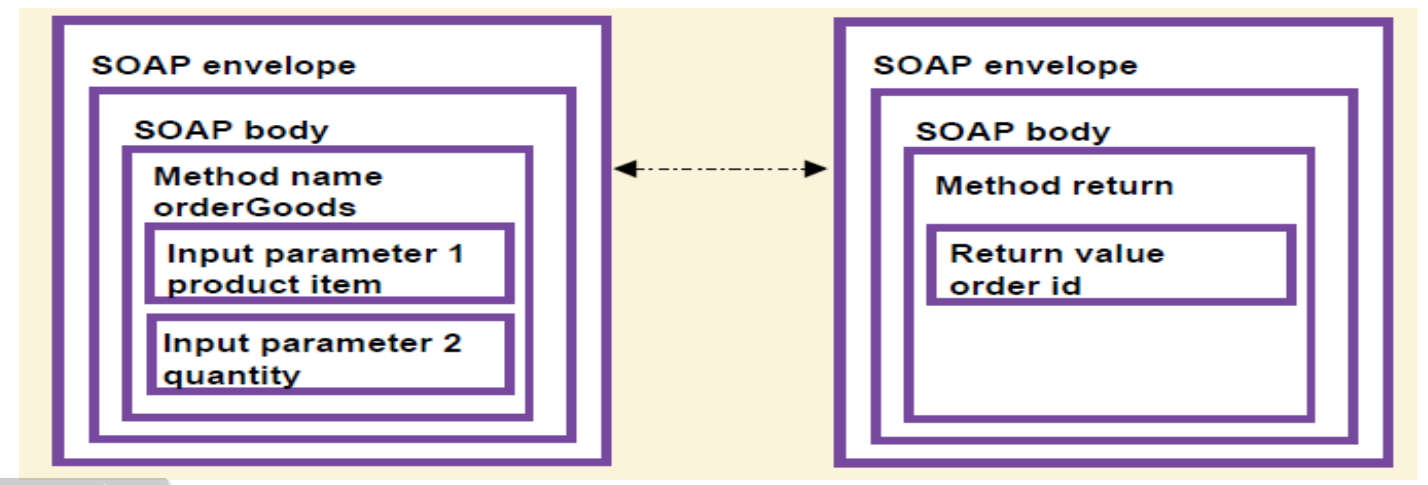
\includegraphics[width=13cm]{./img/04/soap-rpc}
 \caption{\label{pic:soap-rpc} Example of a SOAP RPC exchange.}
\end{figure}
This kind of procedure (same for XML-RPC) requires a request-response cycle. This often leads to longer ``conversations''. The RPC-style is being quickly superseded by newer and more user-friendly technologies.\\\\
In {\bf RPC systems}, the design emphasis is on {\bf verbs}. It uses functions such as {\it getUser()}, {\it addUser()}, etc.


\paragraph{REST}

REST\footnote{REpresentation State Transfer} is a {\bf stateless} client/server protocol. The principles are:
\begin{enumerate}
 \item Each message in the protocol contains all the information needed by the receiver to understand and/or process it. This constraint attempts to {\it ``keep things simple''} and avoids needless complexity.
 \item Set of Uniquely Addressable Resources
 \begin{itemize}
  \item {\it ``Everything is a Resource''} in a RESTful system
  \item Requires universal syntax for resource identification, {\it e.g.} URI.
 \end{itemize}
 \item Set of Well-Defined Operations that can be applied to all resources
 \begin{itemize}
  \item In the context of HTTP (REST APIs), the primary methods are: \\
  {\bf POST}, {\bf GET}, {\bf PUT}, and {\bf DELETE} \\
  These are similar (but not exactly) to the database notion of CRUD (Create, Read, Update, and Delete)
 \end{itemize}
 \item The use of Hypermedia both for Application Information and State Transitions
 \begin{itemize}
  \item Resources are typically stored in a structured data format that supports hypermedia links, such as XHTML or JSON.
 \end{itemize}
\end{enumerate}
In {\bf REST systems}, the design emphasis is on {\bf nouns}. It uses the HTTP Protocols (POST, GET, PUT, and DELETE) a {\it User}, a {\it Location}, etc. 

\clearpage




